% -------------------------------------------------------------------------------- %

\begin{exercise}[\hl{Exercise 7.2: Implementation Task -- n-step Algorithm}]

With an n-step method, the value estimates do change from step to step,
so an algorithm that used the sum of TD errors (see previous exercise) in
place of the error in (7.2) would actually be a slightly different algorithm.
Would it be a better algorithm or a worse one? Devise and program a small
experiment to answer this question empirically.

\end{exercise}

% -------------------------------------------------------------------------------- %

\begin{solution}

We reuse the 19-state random walk process seen in Example 7.1.
For small $n$ the difference between the algorithms is as expected low
(for $n = 1$ they constitute the same algorithm), but for increasing $n$ the
performance of the sum of TD errors algorithm drops relative to the standard algorithm.

\begin{figure}[H]
    \centering
    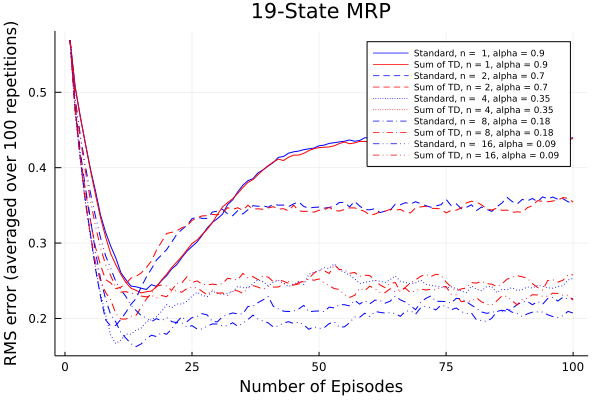
\includegraphics[width = 0.8 \textwidth]{6.2.png}
\end{figure}


\end{solution}

% -------------------------------------------------------------------------------- %
